With both MPI and CUDA independently implemented, the project can test and verify the performance scaling on various configurations. The three testable configurations are CUDA, MPI and MPI+CUDA.


\begin{figure}[!htb]
    \minipage{0.49\textwidth}
    \centering
    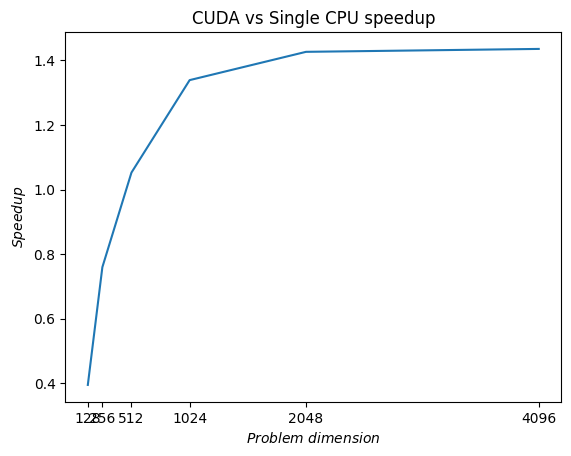
\includegraphics[height=5cm]{images/CUDA_speedup.png}
    \caption{Speedup of using CUDA on different problem sizes.}
    \endminipage\hfill
    \minipage{0.49\textwidth}
    \centering
    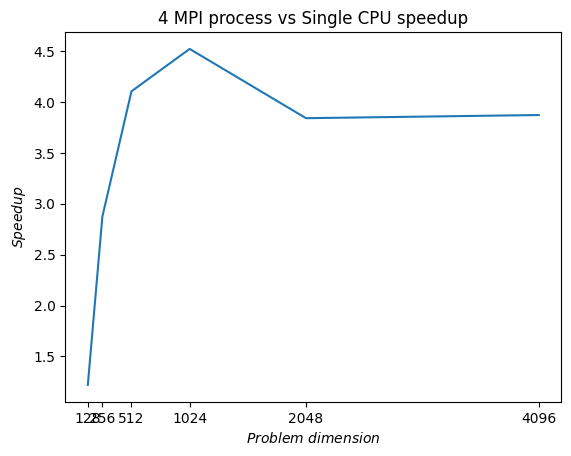
\includegraphics[height=5cm]{images/MPI_speedup.png}
    \caption{Speedup of using 4 MPI processes on different problem sizes.}
    \endminipage\hfill
    \centering
    \minipage{0.49\textwidth}
    \centering
    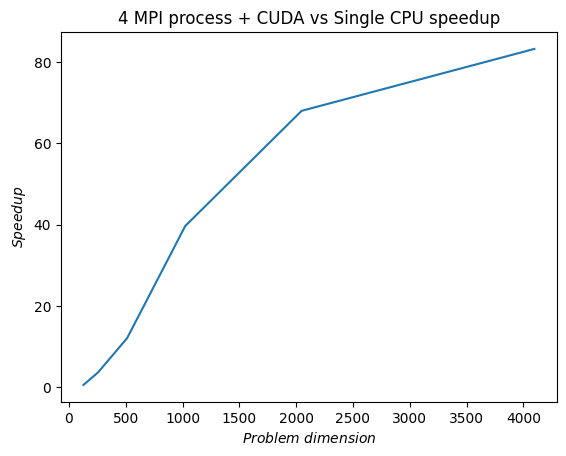
\includegraphics[height=5cm]{images/MPI_CUDA_speedup.png}
    \caption{Speedup of using 4 MPI processes with CUDA on different problem sizes.}
    \endminipage\hfill
\end{figure}

As can be seen from the graphs above, the speedup of CUDA has a positive relation with the problem size. This is a result of optimal warp scheduling since more blocks can be allocated to the same problem and allowing the warp scheduler to keep GPU utilization high. Calculation dependency requirements are limited to local regions and it allows a higher number of blocks to be allocated to the problem for propagation. 

Early implementation of the algorithm only used one single block and threading to allow parallel propagation without loops, but the speedup was limited the speedup to around 42\% but enabling more than one block showed the most prominent speedup.

On the MPI performance, it is apparent that the overhead of collecting the final map to the CPU is significant in smaller problem sizes. Curiously, at problem size of around 1024, the performance gain is greater than the number of processes allocated for the task. This could be the result of splitting the map into sections that limited divergence and increased the rate of wave function collapse which can reduce the number of calls to the random number generator.

When combined, the speedup efficiency of CUDA diminishes as the problem size per GPU decreases and communication overhead from MPI increases. However, MPI+CUDA still shows some performance improvement over single GPU implementation albeit at a lower scaling efficiency.

On performance increase as the number of processors increases, the CPU-only implementation is compared against single CPU implementation, and the MPI+CUDA implementation is compared against single GPU implementation. Both the MPI+CPU version and the MPI+CUDA version are tested with a constant problem size of 8192. 

\begin{figure}[!htb]
    \minipage{0.49\textwidth}
    \centering
    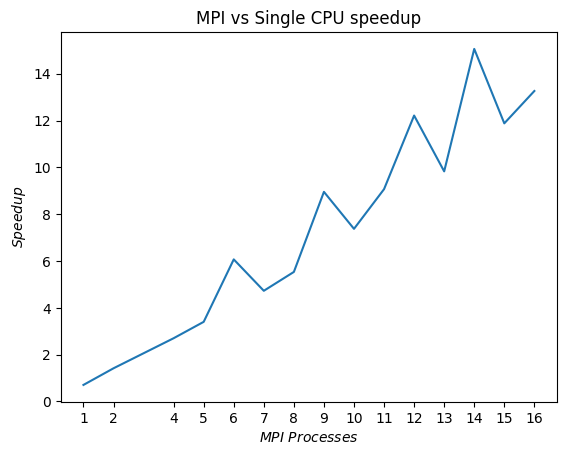
\includegraphics[height=5cm]{images/MPI_speedup_more_processes.png}
    \caption{Speedup of MPI on different number of processes.}
    \endminipage\hfill
    \minipage{0.49\textwidth}
    \centering
    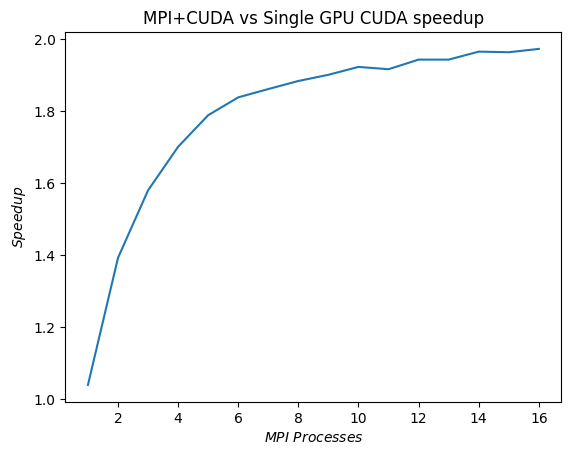
\includegraphics[height=5cm]{images/MPI_CUDA_speedup_more_processes.png}
    \caption{Speedup of MPI+CUDA on different number of processes.}
    \endminipage\hfill
    
\end{figure}

As shown above, the scaling efficiency of this MPI algorithm on CPU is high with almost linear scaling when problem size is large. 

The CUDA-aware version shows that the MPI implementation can lower the speedup in CUDA implementation by lowering the problem size per GPU. Although this indicates that the speedup of using MPI+CUDA is far less prominent than CUDA alone, MPI is still a powerful addition to this algorithm since CUDA performance will drop sharply if the map size exceeds the GPU memory.

In general, using a small number of CUDA-aware MPI processes are favorable in terms of scaling efficiency and reducing overhead.